\chapter{基于纯视觉的体积测算方法研究}
\label{cha:chap4}
\section{引言}
\label{sec:4.1}
利用三维重建的技术流程,可以通过输入二维图片序列的方式获取到场景中的三维稀疏点云或者稠密点云,以视觉的方式来表达场景中的信息。
虽然这些点云可以描绘出空间中的信息,但是还存在以下两个这些问题需要解决:

1)	在三维重建的过程中,由于点云坐标系都是以第一帧的相机为参考坐标系,因此点云坐标系和真实世界坐标系无法对应,对于很多实际应
用场景,都需要获取到该场景的实际水平面,来进行下一步的导航和定位;

2)	由于是单目相机,无法获取特征点的深度信息,因此对于构建出的三维重建点云没有一个绝对尺度的概念。

在解决上述两个问题的基础上,可以对空间中的封闭物体进行高度,面积或者体积的测算,对比传统方法中用激光雷达等设备来测算体积的方
式,现在就可以通过单个摄像头以纯视觉的方式来完成上述过程,并获取到一个精确的结果。本章将以三维重建的点云结果为基础,为了解决
点云的尺度问题,以及求解三维点云的水平面方程,本文将在场景中引入Aruco二维码,因为Aruco二维码本身携带尺度信息,每一种二维码
都有唯一的ID值,并且其还具备较为容易检出的角点坐标。在获取到尺度和水平面方程后,随后结合点云信息可以再进一步计算三维场景的体
积,具体流程如图~\ref{fig:getVolume}所示。

\begin{figure}[H] % use float package if you want it here
    \centering
    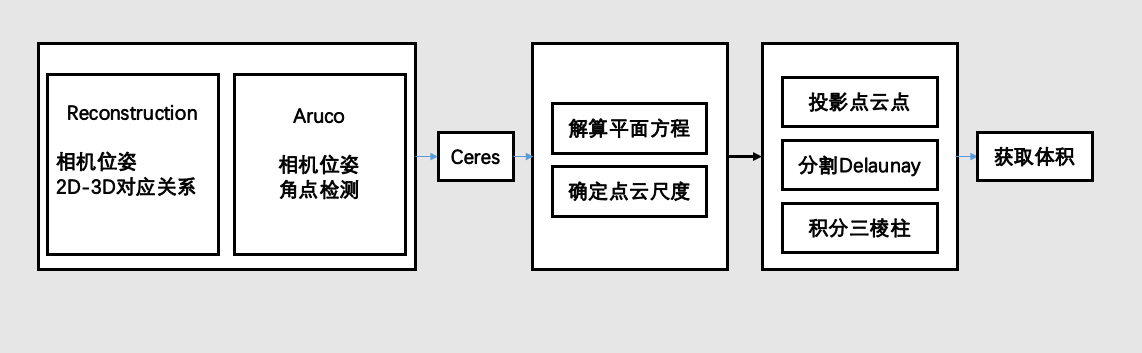
\includegraphics[height=5cm]{getVolume.png}
    \caption{体积测算流程图}
    \label{fig:getVolume}
  \end{figure}

\section{解析水平面方程的一般方法}
\label{sec:4.2}
对于大尺度的场景,都需要得到该场景的水平面所在的平面的方程,由于物体的遮挡,水平面很难直接通过视觉的方法构建出来,从而
导致整个场景非闭合,因此添加水平面后可以使得整个场景封闭;因此,水平面的存在能够更好的计算场景的几何特性,例如场景的高度,
面积,体积等。由于三维重建本身的点云结果都是基于参考坐标系,没有和世界坐标系对齐,本文考虑到可以结合点云中能够获取到世界坐标
系的Aruco二维码作为媒介,进行坐标系的转换,该类型二维码如图~\ref{fig:getVolume_Aruco}所示。
\begin{figure}[H] % use float package if you want it here
  \centering
  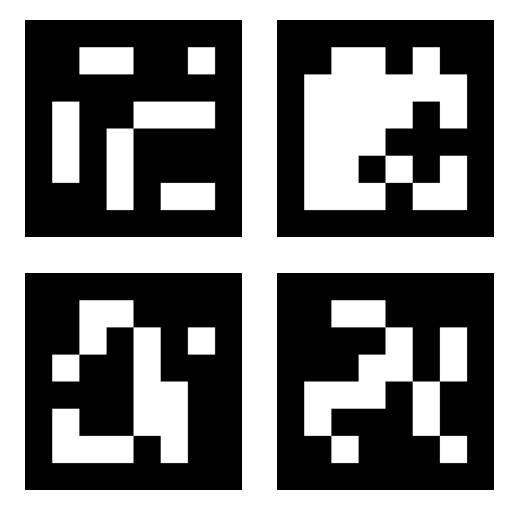
\includegraphics[height=9cm]{getVolume_Aruco.png}
  \caption{多种Aruco示意图}
  \label{fig:getVolume_Aruco}
  \end{figure}
\subsection{检测2D点坐标}
\label{sec:4.2.1}
如图~\ref{fig:getVolume_Aruco_detect}所示,可以利用二维码检测算法检测出场景中二维码的ID值,位置,大小,角点坐标等信息,因为在场景中,
Aruco二维码的布置都会有下侧两个角点直接落在水平面上,因此可以认为所有二维码的下侧角点所构成的平面即是场景的水平面。那么接下
来即可将水平面的求解转化为二维码角点所在平面的求解。在检测的过程中,需要将所有2D图片的索引和角点的位置记录下即可。

\begin{figure}[H] % use float package if you want it here
\centering
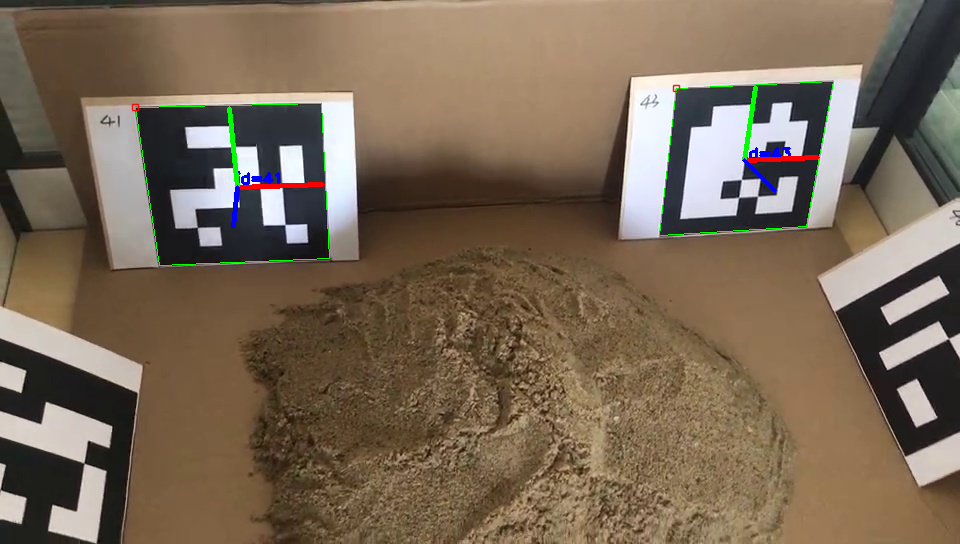
\includegraphics[height=8cm]{getVolume_Aruco_detect_1.png}
\caption{Aruco二维码检测示意图}
\label{fig:getVolume_Aruco_detect}
\end{figure}

\subsection{寻找对应3D坐标}
\label{sec:4.2.2}
在上一小结中,可以获得连续视频帧中每一帧的Aruco二维码下侧两个角点的坐标值,同样的,可以直接将这些包含二维码的视频帧序列作为
三维重建的输入以获取场景的点云,考虑到Aruco的角点被作为特征点时极易被检出,因此只需要通过稀疏点云,即可获取角点在二维图像中
的坐标和三维重建点云中的三维坐标之间的对应关系。

在三维重建的过程中,可以获取到每一帧图像中所有特征点所对应的三维重建点云中的三维坐标,无论是稠密点云或者稀疏点云,都可以得到
一个对应关系,但是考虑到遍历的效率问题,则选择稀疏点云中的点击作为遍历对象。在寻找对应关系的实际过程中,会遇到二维坐标无法映
射到三维坐标点的情况,那么则会优先选择距离二维点坐标欧氏距离最近的点作为替代对象。此外,还需要注意的是,若所布置的Aruco二维
码的所有下侧点都位于同一条直线上,那么这样就无法获取准确的水平面方程,因为经过同一直线的平面并不唯一,因此在布置坐标的过程中
需要注意将所有Aruco二维码尽可能对立放置。
\subsection{平面方程解析}
根据上述两个步骤,可以将待求的水平面方程问题转化成求解N个三维点所在水平面方程的非线性优化问题。本文选择谷歌开源的Ceres solver
库作为解决该非线性问题的工具,Ceres可以解决边界约束鲁棒非线性最小二乘法优化的问题,表达式如下
\begin{equation}
\begin{array}{l}\underset x{min}\;\;\frac12\sum\rho_i(\parallel f_i(x_{i_1},...,x_{i_k})\parallel^2)
\\s.t.\;\;l_j\leq x_j\leq u_j\\\end{array}
\end{equation}
其中$rho_i(\parallel f_i(x_{i_1},...,x_{i_k})\parallel^2$这一部分为残差块, $f_i(.)$为代价函数,代价函数的求解依赖于一系列
参数$[x_{i_1},...,x_{i_k}]$,所有参数构成参数块,限制边界分别为$l_j$,$u_j$。$rho_i$为损失函数,其作用是减少异常值对优化结果的影响。
在利用Ceres解决非线性问题时,通常分为以下三个步骤:\\
1)	构建代价函数,也就是具体问题所对应的目标式,本小结具体解决N个三维点所在水平面的方程;\\
2)	通过代价函数构建待求解的优化问题;\\
3)	配置求解器参数并求解问题,在这一过程中主要是设定求解方程的方式。\\
上述步骤如代码~\ref{code:chap3:get_plane}所示。
\begin{lstlisting}[
  language=C++,
  numbers=left,                
  numberstyle=\footnotesize,
  frame=single,     
  basicstyle=\small\tt,    
  escapeinside = '',
  caption={获取平面方程参数的~C++~实现},
  label={code:chap3:get_plane}]
  vector<vector<float>> plane_data1;
  vector<float> planex_data1 ,planey_data1, planez_data1;'//待优化量'
  '// 第一部分:构建代价函数模型'
  struct CURVE_FITTING_COST_plane
  {
    CURVE_FITTING_COST_plane (double x,double y,double z)
    :_x( x ), _y ( y ), _z ( z ) {}
    '// 残差的计算'
    template <typename T>
    bool operator() (
      const T* const plane,    
      T* residual ) const 
    {
      residual[0] = plane[0]*T(_x) + plane[1]*T(_y) 
                  + plane[2]*T(_z) + plane[3]; 
      return true;
    }
    const double _x, _y, _z;
  };

  int main ( int argc, char** argv )
  {   
    double plane[4] = {0.1,0.1,0.2,0};
    '// 第二部分:构建最小二乘问题'
    ceres::Problem problem2;
    for ( int i=0; i<planex_data1.size(); i++ ){
      problem2.AddResidualBlock 
      (new ceres::AutoDiffFunction<CURVE_FITTING_COST_plane,1,4> 
      (new CURVE_FITTING_COST_plane 
      (planex_data1[i], planey_data1[i],planez_data1[i])),
      nullptr,
      plane);
    }
    '// 第三部分:配置求解器'
    ceres::Solver::Options options2;    
    options2.linear_solver_type = ceres::DENSE_QR;
    options2.minimizer_progress_to_stdout = true; 
    ceres::Solver::Summary summary2;                 
    ceres::Solve ( options2, &problem2, &summary2 );
    for ( auto a:plane ) {
      outfile_kabc<<a*1/plane[3]<<endl;
      }
    return 0;
  }
\end{lstlisting}
对于任意平面方程,都可以利用以下方程通过确定4个参数的方式来确定唯一解析解。
\begin{equation}ax+by+cz+d= 0\end{equation}
在迭代的过程中,同时需要确定每个带估计参数的初始值,最终可以得到方程的四个参数a,b,c,d。

\section{解算尺度}
\label{sec:4.3}
由单目视觉重建出来的点云地图都存在没有一个确定尺度的问题,地图中的特征点坐标和相机的位姿都是相对尺度,即最常见的采取初始化成
功后的前两帧作为单位尺度,后续的所有关键帧都以此为参考确定尺度。这样的做法可以获取到地图中所有描述的绝对尺度,但无法计算出实
际尺度,本文通过在场景中引入已知尺度的二维码来确定所构点云地图的真实尺度,主要针对同一场景,通过计算两种SLAM的相机位姿来确定
相对尺度和绝对尺度之间的比例,从而确定绝对尺度。
\subsection{计算绝对尺度和相对尺度}
首先,获取绝对尺度的数据,由图~\ref{fig:getVolume_Aruco_detect}所示同时可以得到相机在某一个确定的Aruco下的位姿,因为二维
码自带确定的边长信息,因此可以得到带有绝对尺度的相机位姿($T_x$,$T_y$,$T_z$)。在实际的工程中需要注意,必须选择不同状态的
相机在同一二维码下的位姿,则可以通过多个图像序列获取到多个不同位姿。

其次,再获取同一批图像序列的相对尺度,通过三维重建的结果,就可以得到每一帧相机在参考坐标系下的位姿($T_x$,$T_y$,$T_z$),
该位姿为相对尺度,因为只需要考虑到尺度的大小关系,因为不需要讨论不同坐标系之间的相对转化问题。
\subsection{尺度估计方法}
通过上一小节,可以获取到多个针对同一场景的两种SLAM相机位姿估计结果,因为两种SLAM方法估计出的相机位姿是基于不同的坐标系得到
的,本文提出利用相机在不同坐标系下移动的欧式距离之间的比例来确定尺度,简化公式为:
\begin{equation}K\;=\;\frac{\triangle Pose_{rel}}{\triangle Pose_{abs}}  
\label{equ:getVolume_K}\end{equation}
同4.2.1节,利用Ceres库得到最优解K值,计算如代码~\ref{code:chap3:get_k}所示,
\begin{lstlisting}[
  language=C++,
  numbers=left,                
  numberstyle=\footnotesize,
  frame=single,     
  basicstyle=\small\tt,    
  escapeinside = '',
  caption={获取尺度值的~C++~实现},
  label={code:chap3:get_k}]
  vector<vector<float>> colmap, opencv;
  vector<float> colmap_data1 ,opencv_data1;'//待优化量'
  '// 第一部分:构建代价函数模型'
  struct CURVE_FITTING_COST_k
  {
    CURVE_FITTING_COST_k (double x,double y)
    '// 残差的计算'
    template <typename T>
    bool operator() (
      const T* const k,     
      T* residual ) const     
    {
      residual[0] = T ( _y ) - ( k[0]*T ( _x ) ); // y-ax
      return true;
    }
    const double _x, _y;
  };
  int main ( int argc, char** argv )
  {   
    double k[1] = {0};
    '// 第二部分:构建最小二乘问题'
    ceres::Problem problem;
    for ( int i=0; i<colmap_data1.size(); i++ ){
      problem.AddResidualBlock 
      (new ceres::AutoDiffCostFunction<CURVE_FITTING_COST_k, 1, 1>
      (new CURVE_FITTING_COST_k 
      (opencv_data1[i], colmap_data1[i])),
      nullptr,
      k);
    }
    '// 第三部分:配置求解器'
    ceres::Solver::Options options;   
    options.linear_solver_type = ceres::DENSE_QR;  
    options.minimizer_progress_to_stdout = true;  
    ceres::Solver::Summary summary;              
    ceres::Solve ( options, &problem, &summary );  
    for ( auto a:k ) {
      outfile_kabc<<a<<endl;
      }
  return 0;
  }
\end{lstlisting}
只需要杰出唯一参数K即可,在计算的过程中需要随机获取任意两帧之间的位姿,以减小误差。
\section{解算体积}
\label{sec:4.4}
内容内容内容内容内容内容内容内容内容内容内容内容内容内容内容

